\subsection{\secState{R}Detected Obstacles}\label{s:detectedObstacles}
\paragraph{Idea:} The \emph{visibility} inside avoidance grid and \emph{obstacle} probability are interconnected for most ranging sensors (ex. LiDAR). The goal of this section is to introduce \emph{visibility hindrance} concept which includes space uncertainty assessment and detected obstacle  processing.

\paragraph{Detected Obstacle Rating:} The \emph{detected obstacle rating} defines UAS chances to encounter detected obstacle in avoidance grid $cell_{i,j,k}$. Final \emph{detected obstacle rating} is merged information (eq. \ref{eq:detectedObstacleRatingForCell}). The \emph{sensor field} can contain \emph{multiple} \emph{static obstacle sensors}.

\paragraph{Detected Obstacle Rate for LiDAR:},Lets have only one sensor set as homogeneous two axis rotary LiDAR. For one $cell_{i,j,k}$ there exists set of passing LiDAR beams:

\begin{equation}\label{eq:lidarRaysTroughCell}
    lidar Rays(cell_{i,j,k})=
    \left\{
        \begin{aligned}
        \left[
            \begin{gathered}
                horizontal^\circ\in horizontal Offsets,\\
                vertical^\circ\in vertical Offsets
            \end{gathered}
        \right]\in\R^2:&\\
        horizontal^\circ\in cell_{i,j,k}.horizontal &Range,\\
        vertical^\circ\in cell_{i,j,k}.vertical &Range\\
        \end{aligned}
    \right\}
\end{equation}

\newpage\noindent The horizontal and vertical offset of LiDAR ray is homogeneous. Meaning the horizontal/vertical distances between each two neighbouring LiDAR beams are equal.

The set $lidar Rays(cell_{i,j,k}))$ (eq. \ref{eq:lidarRaysTroughCell}) is finite countable and nonempty for any $c_{i,j,k}$, otherwise it will contradict   the definition of avoidance grid (def. \ref{def:AvoidanceGrid}).

The hit function $lidarScan()$ returns a distance of single beam return for beam with dislocation $[horizontal^\circ,$ $vertical^\circ]$ $\in$ $lidar Rays(cell_{i,j,k})$ angle offsets. The set of LiDAR hits (eq. \ref{eq:lidarHitFunction}) in cell $cell_{i,j,k}$ is defined like follow:

\begin{equation}\label{eq:lidarHitFunction}
    lidar Hits(cell_{i,j,k})=\left\{
        \begin{aligned}
        \left[
            \begin{gathered}
                distance=lidar Scan(),\\
                horizontal^\circ\in horizontal Offsets,\\
                vertical^\circ\in vertical Offsets
            \end{gathered}
        \right]\in\R^2:&\\
        distance \in cell_{i,j,k}.distance &Range,\\
        horizontal^\circ\in cell_{i,j,k}.horizontal &Range,\\
        vertical^\circ\in cell_{i,j,k}.vertical &Range\\
        \end{aligned}
    \right\}
\end{equation}

\noindent The \emph{naive} obstacle rate in case of LiDAR sensor defined as ratio between landed hits and possible hits:

\begin{equation}\label{eq:naiveObstacleRate}
    obstacle^{LiDAR}_{cell_{i,j,k}}=\frac{lidar Hits(cell_{i,j,k})}{lidar Rays(cell_{i,j,k})}
\end{equation}

\begin{note}
    The \emph{naive obstacle rate} (eq. \ref{eq:naiveObstacleRate}) ignores that \emph{LiDAR rays} are getting more far apart from each other. The \emph{cell surface} is increasing with cell distance from \emph{UAS}.
\end{note}

\noindent The hindrance (eq. \ref{eq:probabilityOfVisibilityHindrance}) rate is naturally defined as supplement to naive obstacle rate. This definition is sufficient, because its reflecting the \emph{remaining sensing capability} of  LiDAR.

\begin{equation}\label{eq:probabilityOfVisibilityHindrance}
    hindrance^{LiDAR}_{cell_{i,j,k}}=1-\frac{lidar Hits(cell_{i,j,k})}{lidar Rays(cell_{i,j,k})}
\end{equation}

\paragraph{Cell Density Function:}  Let`s start with differential form of cell surface (eq. \ref{eq:finalCellSquare}). The target object have several hits in \emph{Avoidance Grid}. Target $cell_{i,j,k}$ has following properties which are used in surface calculation:
\begin{enumerate}
    \item \textit{Horizontal span} - defines range of horizontal scanner partition.
    \item \textit{Vertical span} - defines range of vertical scanner partition.
\end{enumerate}

\newpage\noindent By rewriting (eq. \ref{eq:finalCellSquare}) and using horizontal range parameter and inverted vertical range parameter following surface integral is obtained (eq. \ref{eq:cellSurfaceIntengralDelta}).

\begin{multline}\label{eq:cellSurfaceIntengralDelta}
    Area(cell_{i,j,k}) =\\ \int_{horizontal_{start}^\circ}^{horizontal_{end}^\circ}\int_{vertical_{end}^\circ}^{vertical_{start}^\circ} radius^2 \cos(vertical^\circ) \quad \text{d} vertical^
    \circ\text{d} horizontal^\circ
\end{multline}

\begin{note}
    The \emph{radius} parameter is \emph{average} distance of hits landed in $cell_{i,j,k}$. This helps to reflect real \emph{scanned surface}.
\end{note}

Numerically stable integration exist for boundaries $horizontal^\circ \ in [-\pi,\pi]$, $vertical^\circ \in [-\frac{\pi}{2},\frac{\pi}{2}]$ given as follow:

\begin{multline}\label{eq:intersectionSurfaceForCell}
    Area(radius,horizontal Range, vertical_{start}^\circ, vertical_{end}^\circ) =\dots\\ 
    =\left\{
    \begin{aligned}
        vertical&_{start}^\circ <0, vertical_{end}^\circ \le 0 :\\ 
            &radius^2(\sin |vertical_{start}^\circ| - \sin|vertical_{end}^\circ|)\times horizontal Range)\\
         vertical&_{start}^\circ <0, vertical_{end}^\circ > 0   :\\
            & r^2(\sin |vertical_{start}^\circ| + \sin|vertical_{end}^\circ|)\times horizontal Range)\\
         vertical&_{start}^\circ \ge 0 vertical_{end}^\circ < 0 :\\
            & r^2(\sin vertical_{end}^\circ- \sin vertical_{start}^\circ)\times horizontal Range)
    \end{aligned}
    \right.
\end{multline}

\noindent An intersection surface for cell is defined in (eq. \ref{eq:intersectionSurfaceForCell}). Area covered by LiDAR hits (eq. \ref{eq:lidarHitArea}) is defined as LiDAR hit rate (hits to passing rays ratio) multiplied by \emph{Average} cell intersection surface (eq. \ref{eq:intersectionSurfaceForCell}).

\begin{equation}\label{eq:lidarHitArea}
    lidar Hit Area(cell_{i,j,k}) = \frac{lidar Hits(cell_{i,j,k})}{lidar Rays(cell_{i,j,k})} \times Area\left(\begin{gathered}radius,horizontal Range,\\ vertical_{start}^\circ, vertical_{end}^\circ\end{gathered}\right)
\end{equation}

\noindent There is user defined parameter for \emph{LiDAR treshold area}, which represents minimal considerable surface area for obstacle to be threat. The \emph{detected obstacle rate} considering surface is defined in (eq. \ref{eq:lidarHitFormula}) and it removes bias of naive approach (eq.\ref{eq:naiveObstacleRate}).

\begin{equation}\label{eq:lidarHitFormula}
    obstacle(LiDAR,cell_{i,j,k})=\min\left\{\frac{lidar Hit Area(cell_{i,j,k})}{UAS.lidar Threshold Area},1\right\}
\end{equation}



\newpage\paragraph{Visibility Rate for  LiDAR:} For each $cell_{i,j,k}$ and each sensor in sensor field there exist hindrance rate, which defines how much vision is clouded in single cell. Example of hindrance calculation for LiDAR has been given by (eq. \ref{eq:probabilityOfVisibilityHindrance}). Let us consider cell row $cell Row (j_{fix},$ $k_{fix})$ with fixed horizontal index $j_fix$ and vertical index $k_{fix}$ is given as series of cells (eq. \ref{eq:cellrowDefinition}).

\begin{equation}\label{eq:cellrowDefinition}
    cellRow(j_{fix},k_{fix})= \left\{cell_{i,j,k}\in Avoidance Grid :\begin{aligned}&i\in\{1,..,layersCount\},\\&j=j_{fix}, k=k_{fix}\end{aligned}\right\}
\end{equation}

For each $cell_{i,j,k}$ there exists a function which calculates final visibility hindrance rate. Then for ordered cell row:
\begin{equation*}
    cell Row(j_{fix},k_{fix}) = \{cell_{1,j_{fix},k_{fix}},  cell_{2,j_{fix},k_{fix}}, \dots, cell_{layers Count,j_{fix},k_{fix}}\}    
\end{equation*}
and for one selected $cell_{i,j,k}$ the visibility rate is naturally defined as a supplement to hindrance from previous cells. The visibility is defined in (eq. \ref{eq:FinalVisibilityProbability}).

\begin{multline}\label{eq:FinalVisibilityProbability}
    visibility(cell_{i_c,j_c,k_c})=\dots\\ \dots =1 - \sum_{index\in\N^+}^{index < i_c} hindrance(cell_{a,j_c,k_c}: cell_{a,j_c,k_c}\in cell Row(j_{c},k_{c})
\end{multline}

\paragraph{Example:} Let be $cell_{4,j_{fix},k_{fix}}$ is selected for visibility rate assessment, then $cell_{1,j_{fix},k_{fix}}$, $cell_{2,j_{fix},k_{fix}}$, and $cell_{3,j_{fix},k_{fix}}$, are used as a base of cumulative hindrance rate.

\noindent \emph{The cumulative hindrance rate} for any $cell Row(j_{fix},k_{fix})$ is bounded:

\begin{equation}
    0 \le \sum_{cell\in cell Row(j_{fix},k_{fix})} visibility(cell) \le 1
\end{equation}

\begin{note}
    A \emph{cumulative hindrance rate} does not always reach 1 in case of LiDAR sensor, because some rays may pass or hit after leaving \emph{avoidance grid} range.
\end{note}


\begin{figure}[H]
    \centering
    \begin{subfigure}{0.32\textwidth}
        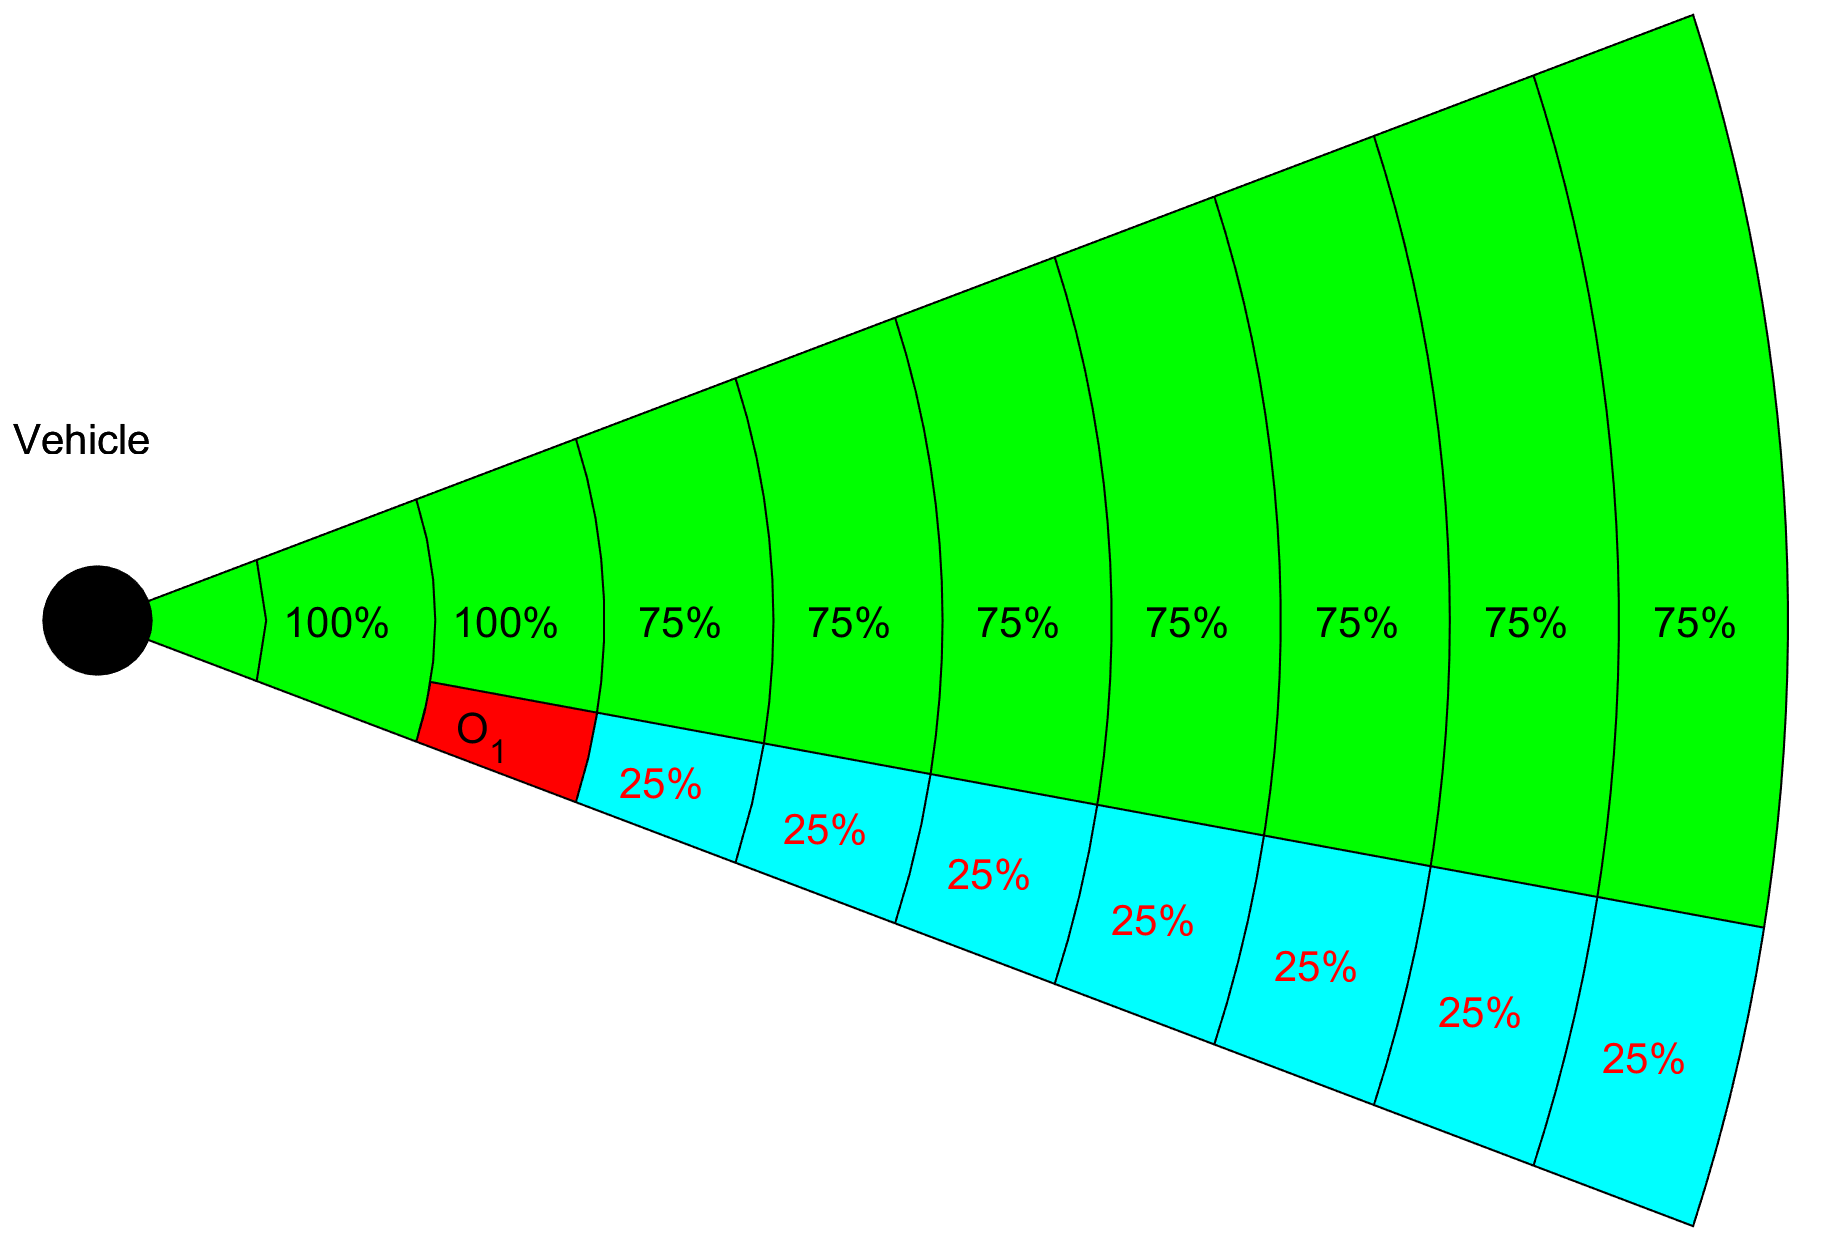
\includegraphics[width=0.9\linewidth]{\FIGDIR/TE006VisibilityFirstObstacle} 
        \caption{1\textsuperscript{st} hindrance.}
        \label{fig:fistObstacleHindrance}
    \end{subfigure}
    \begin{subfigure}{0.32\textwidth}
        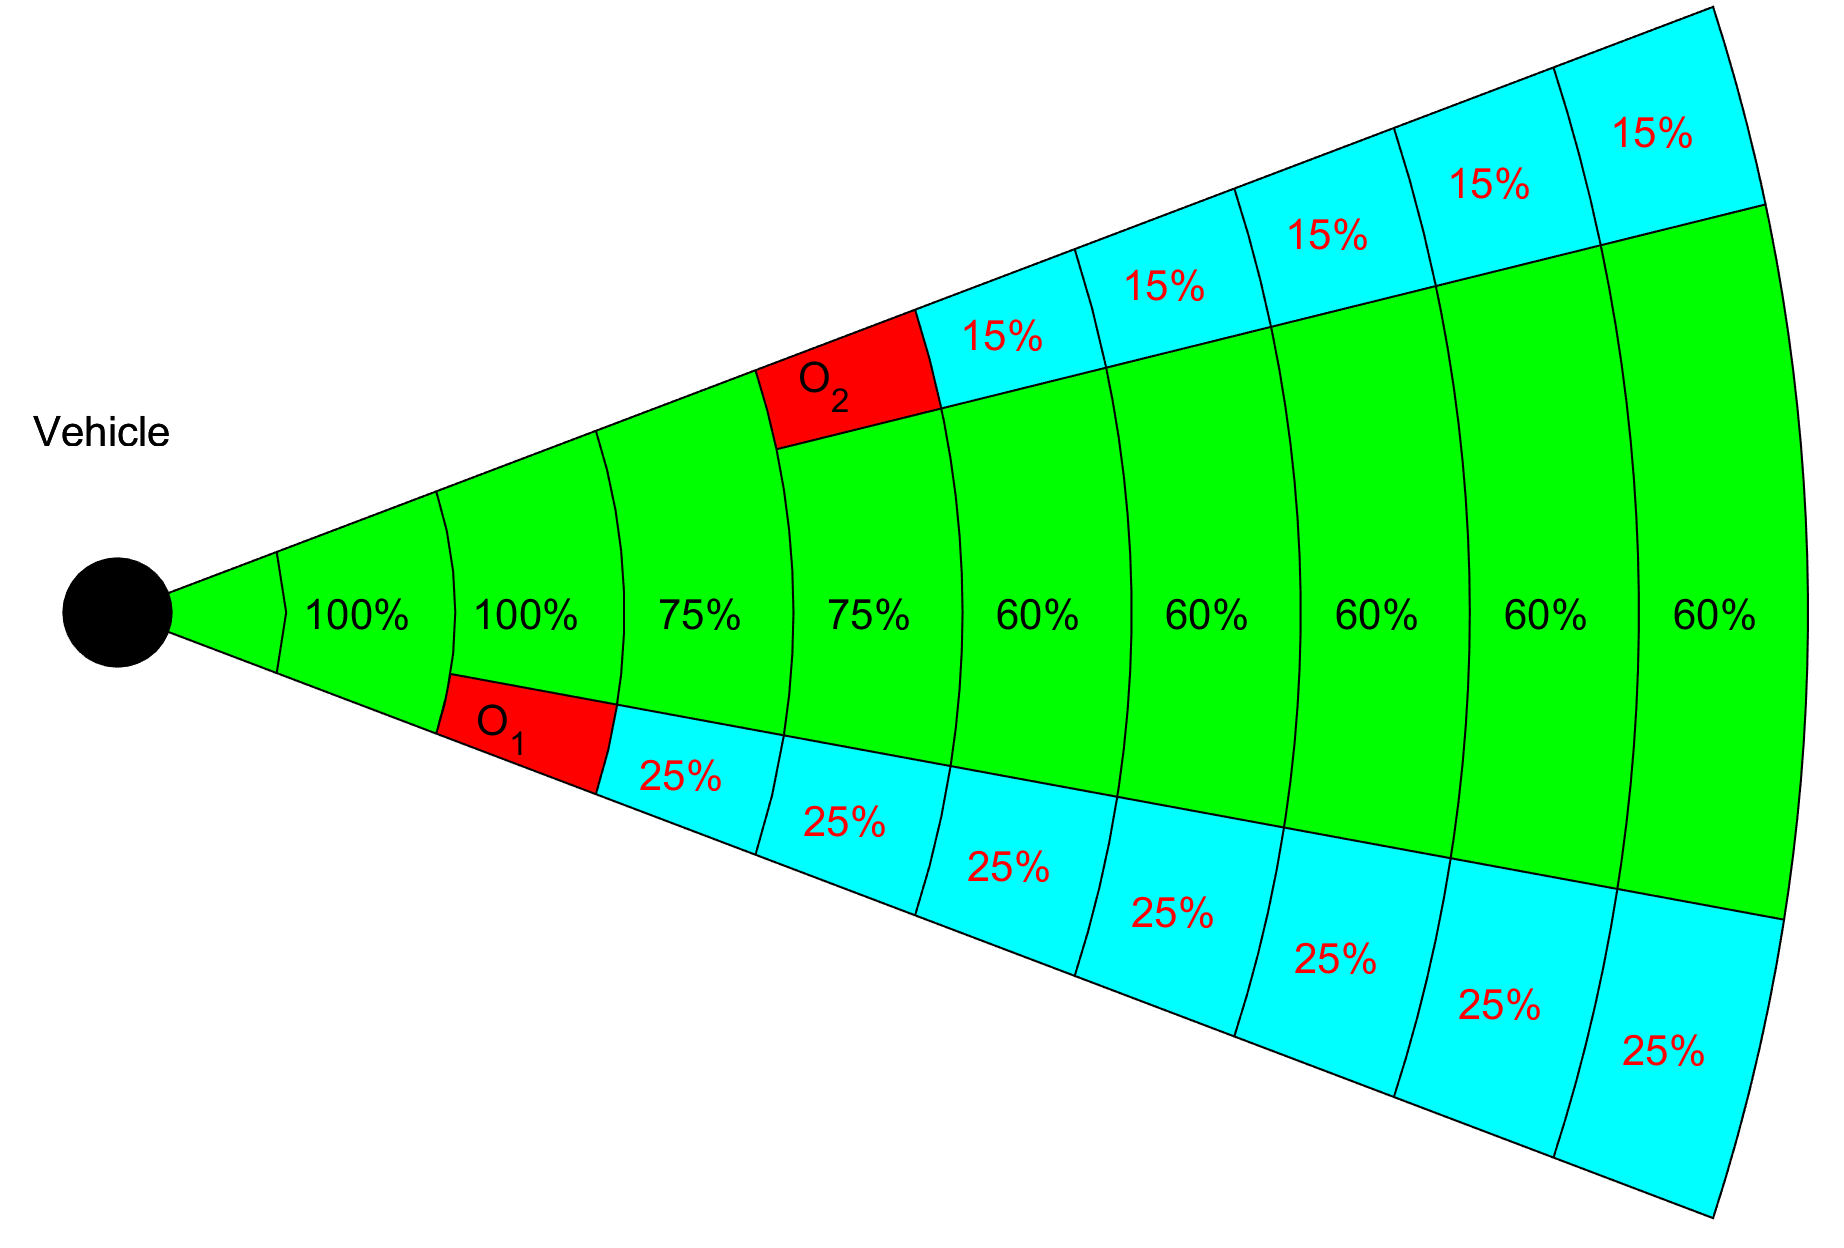
\includegraphics[width=0.9\linewidth]{\FIGDIR/TE007VisibilitySecondObstacle} 
        \caption{2\textsuperscript{nd} hindrance.}
        \label{fig:secondObstacleHindrance}
    \end{subfigure}
    \begin{subfigure}{0.32\textwidth}
        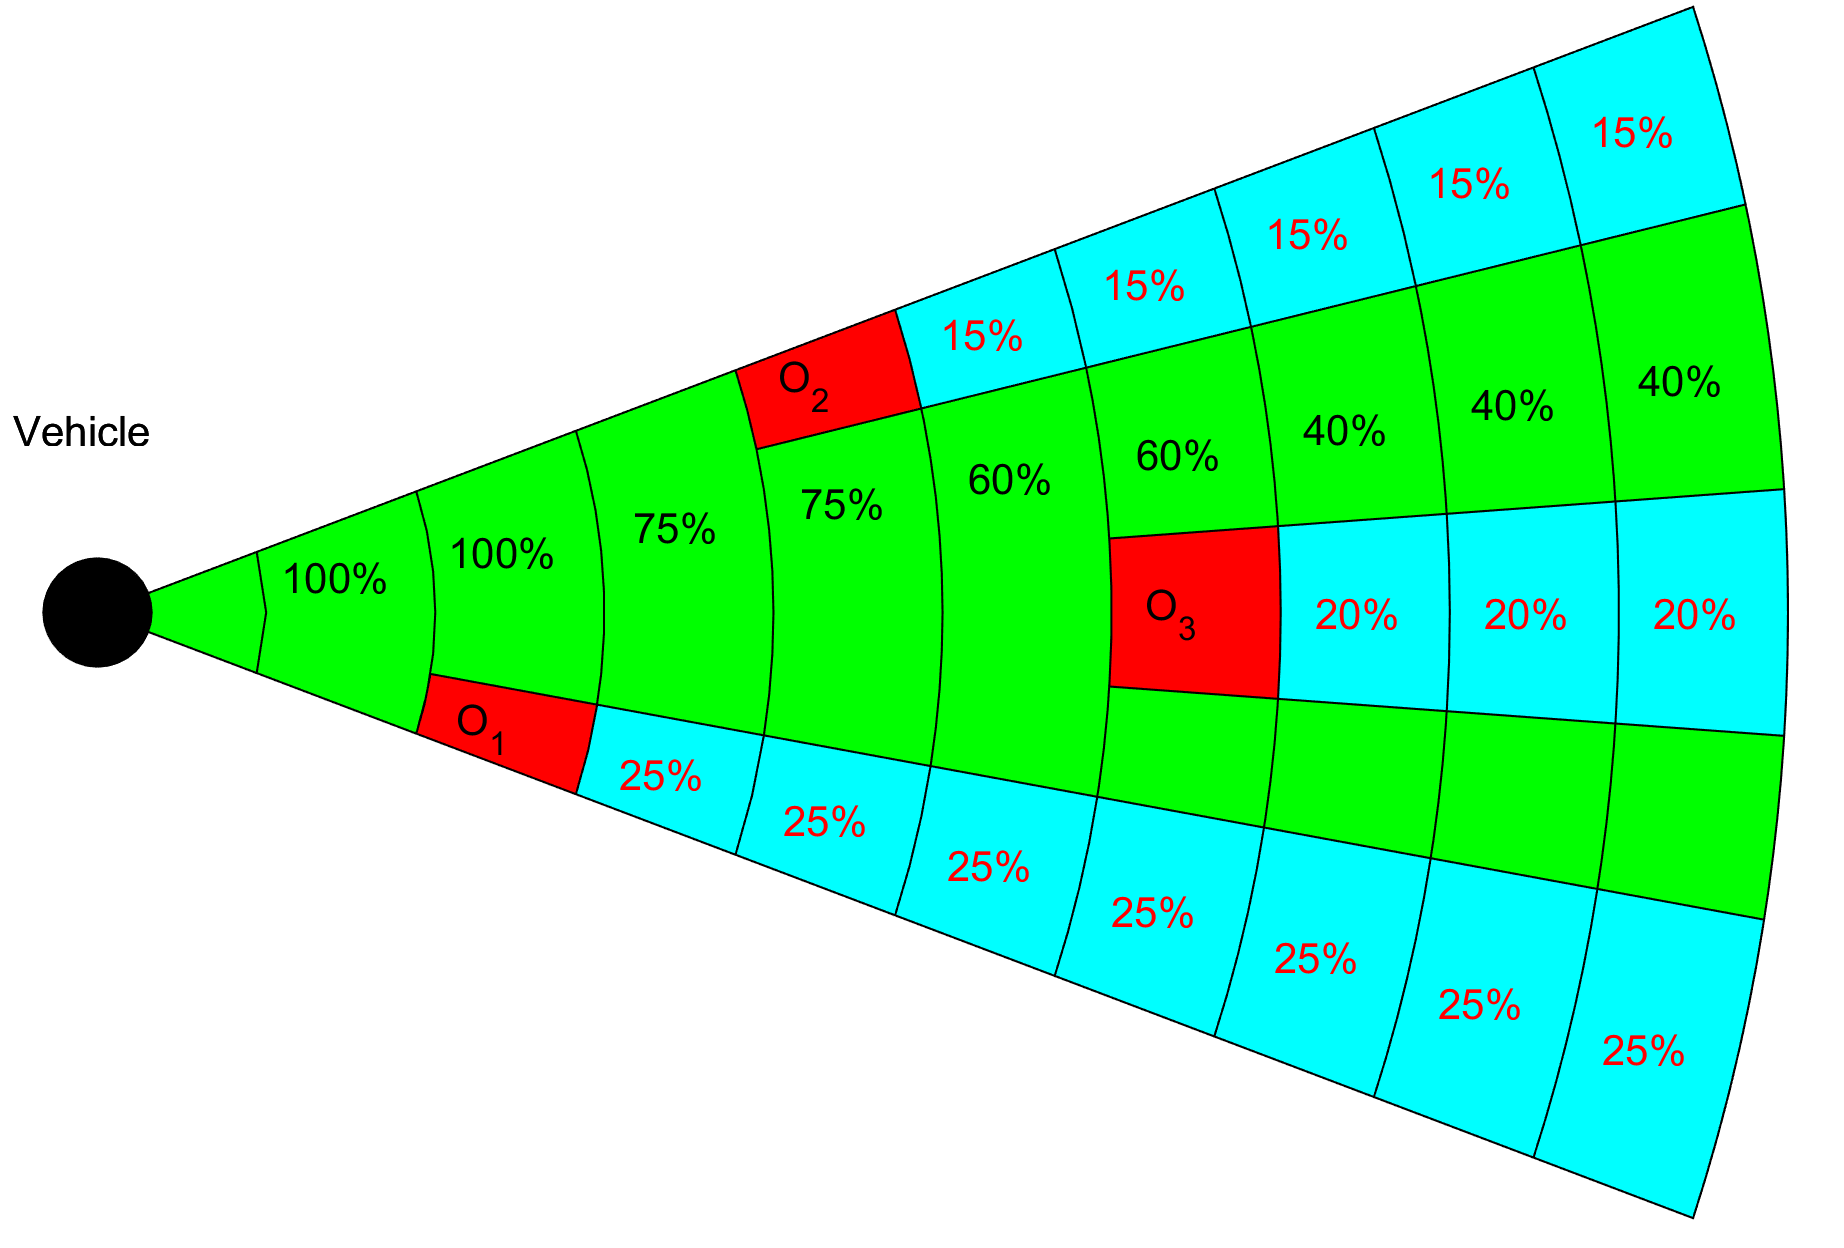
\includegraphics[width=0.9\linewidth]{\FIGDIR/TE008VisibilityThirdObstacle} 
        \caption{3\textsuperscript{rd} hindrance.}
        \label{fig:thirdObstacleHindrance}
    \end{subfigure}
    \caption{Obstacle hindrance impact on visibility in \emph{Avoidance Grid Slice}.}
    \label{fig:hindranceImpactOnVisibility}
\end{figure}

\noindent For one cell row $cell Row(j_{fix},k_{fix})$, where count of layers is equal to 10, and layers have equal spacing. There is LiDAR sensor

\noindent During consequent LiDAR scans $s(t_0)$, $s(t_1)$, $s(t_2)$, and $s(t_3)$ the obstacle sets $\mathscr{O}_1(t_1)=\{o_1\}$, $\mathscr{O}_2(t_2)=\{o_1,o_2\}$, and $\mathscr{O}_3(t_3)=\{o_1,o_2,o_3\}$ are discovered. Assigned hindrance rates are like follow:

\begin{enumerate}
    \item\emph{Time $t_0$} - there is no obstacle nor hindrance, all cells are fully visible.

    \item\emph{Time $t_1$} (fig. \ref{fig:fistObstacleHindrance}) - $\mathscr{O}_1(t_1)=\{o_1\}$ was detected, the hindrance rate  for $cell_{3,j_{fix},k_{fix}})$ is equal to $0.25$. The visibility rate in cells $cells_{4-10,j_{fix},k_{fix}}$ is $0.75$. 
    
    \item\emph{Time $t_2$} (fig. \ref{fig:secondObstacleHindrance}) - $\mathscr{O}_2(t_2)=\{o_1,o_2\}$ was detected, the additional hindrance rate for $cell_{5,j_{fix},k_{fix}}$ is $0.15$. The visibility rate in  $cells_{6-10,j_{fix},k_{fix}}$ is lowered by additional $0.15$ and its set to $0.60$ now.
    
    \item\emph{Time $t_3$} (fig. \ref{fig:thirdObstacleHindrance}) - $\mathscr{O}_3(t_3)=\{o_1,o_2,o_3\}$  was detected the additional hindrance rate for  $cell_{7,j_{fix},k_{fix}}$ is $0.20$. The visibility rate in $cells_{8-10,j_{fix},k_{fix}}$ is lowered by additional $0.20$ and its set to $0.40$  now.
\end{enumerate}